\chapter{Sistemos naudojimo scenarijus}

\section{Esamoji būklė}

Mokyklos būstinėje yra vienas nešiojamas kompiuteris su Windows operacine
sistema, kuriame laikomi visi „einamieji“ duomenys, bei prie jo prijungtas 
lazerinis spausdintuvas. Nuotolinio mokymo mokykla taip pat turi savo 
svetainę, bei duomenų bazę su informacija apie moksleivius ir dėstytojus.
Darbuotojai dirba su savo asmeniniais kompiuteriais, kuriuose naudoja
įvairią programinę įrangą (pavyzdžiui naudojamų operacinių sistemų 
sąraše yra „Windows XP“, „Windows 7“, „Ubuntu Linux“, „Xubuntu Linux“,
„Gentoo Linux“). Dauguma darbuotojų turi didelę darbo su biuro 
programomis patirtį.
% TODO Išversti ir papildyti.

\section{Scenarijaus aprašas}

\ref{fig:uml_usecase} diagramoje pavaizduota darbo su sistema UML schema.



\begin{figure}[htb]
  \begin{center}
    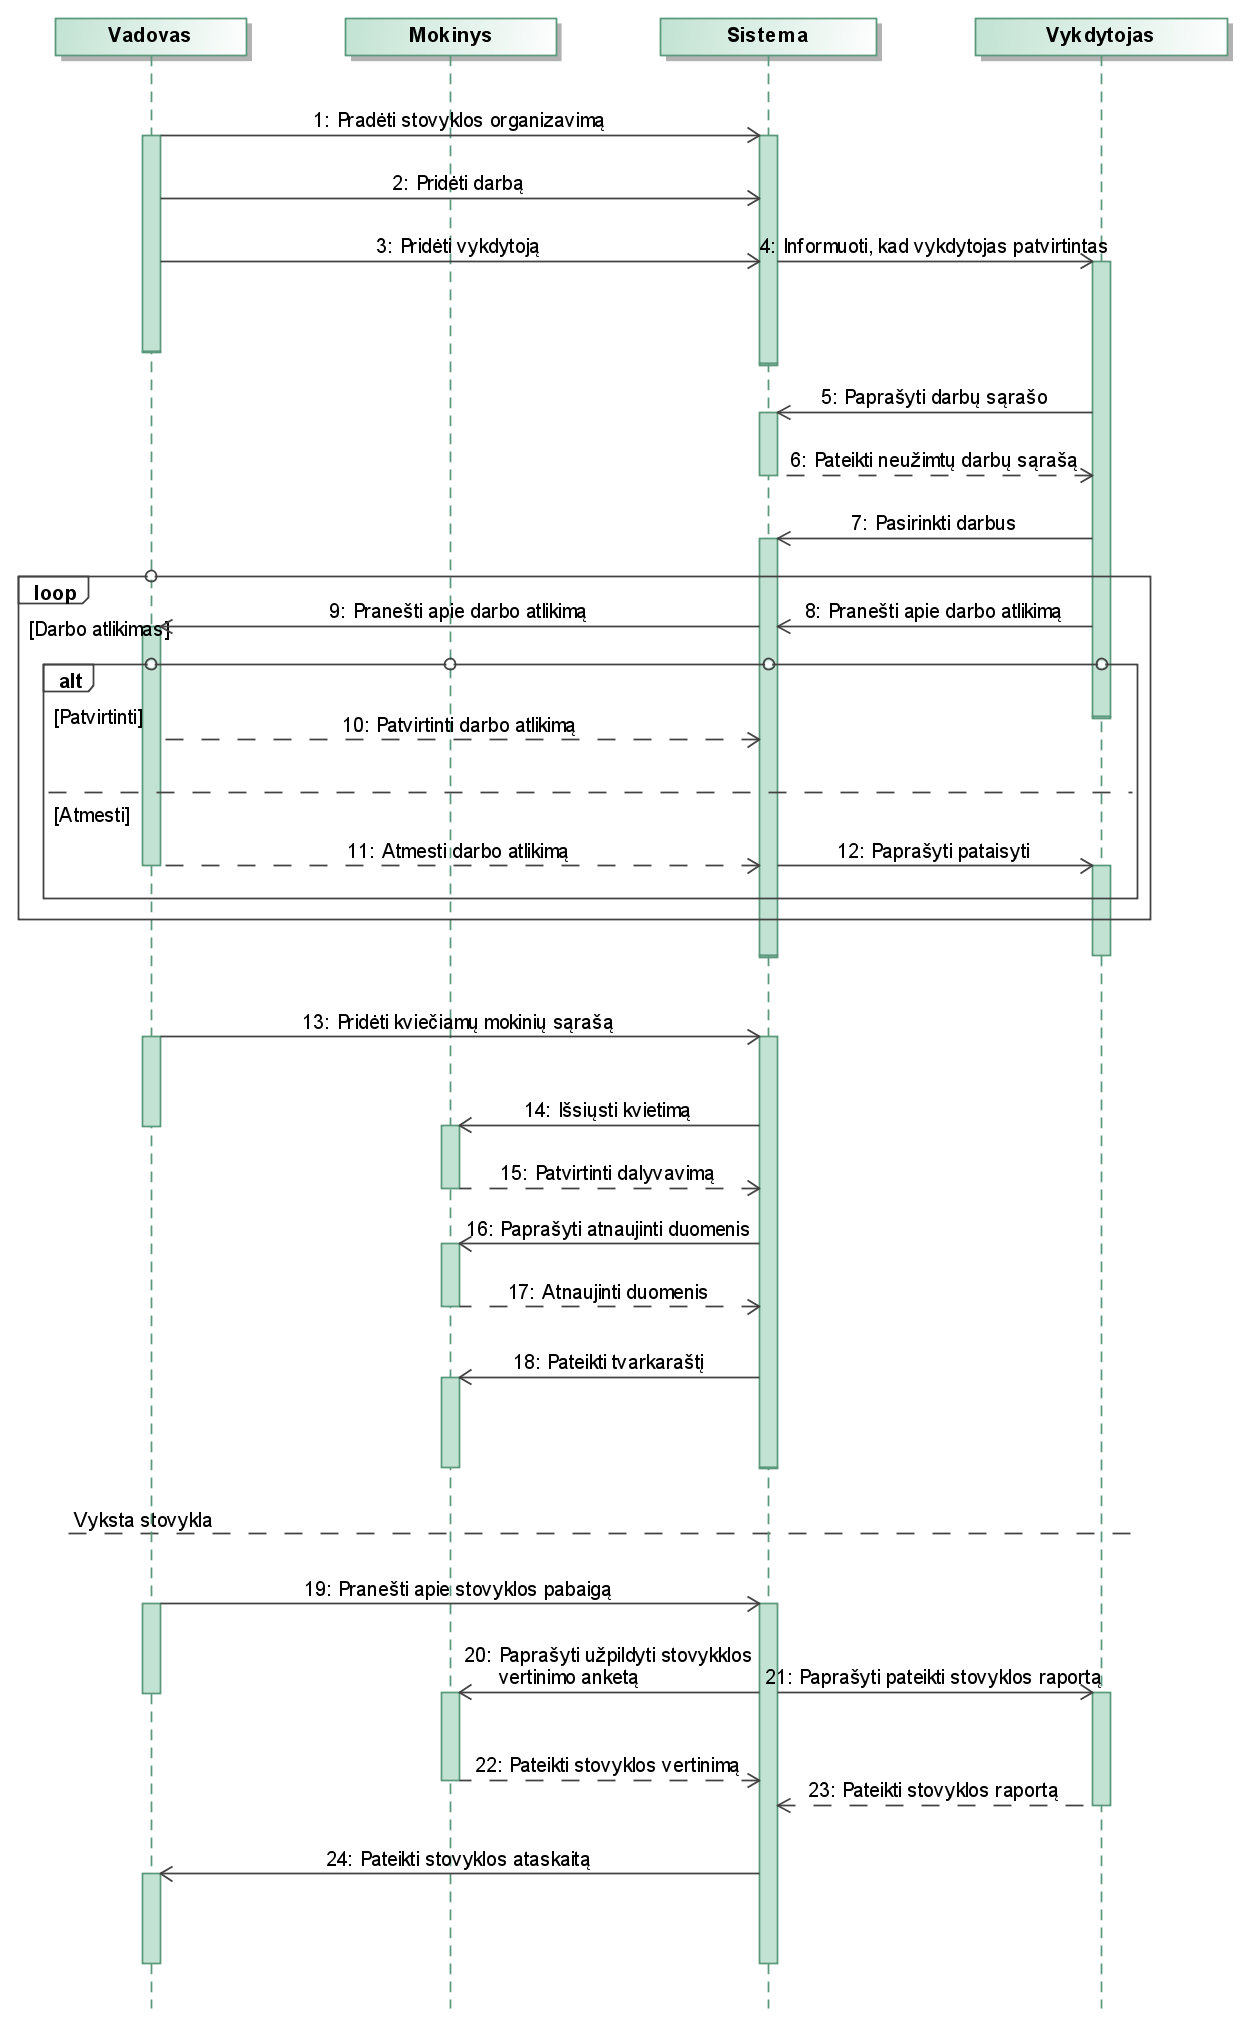
\includegraphics[scale=0.7]{images/Seka.png}
    \caption{UML schema vaizduojanti darbą su įdiegta sistema.}
  \end{center}
  \label{fig:uml_usecase}
\end{figure}


\subsection{Darbo vietų aprašas}
\begin{enumerate}
  \item Vadovas
	\begin{itemize}
	  \item Techninė įranga
		\begin{enumerate}
			\item Kompiuteris su internetu
		\end{enumerate}
	  \item Programinė įranga
		\begin{enumerate}
			\item Operacinė sistema, interneto naršyklė
		\end{enumerate}
	  \item Kvalifikaciniai reikalavimai
		\begin{enumerate}
			\item Kompiuterinio raštingumo pagrindai
			\item Sistemos "Skirstytuvas" administavimo apmokymas % FIXME
		\end{enumerate}
	\end{itemize}

  \item Vykdytojas
	\begin{itemize}
	  \item Techninė įranga
		\begin{enumerate}
			\item Kompiuteris su internetu
		\end{enumerate}
	  \item Programinė įranga
		\begin{enumerate}
			\item Operacinė sistema, interneto naršyklė
		\end{enumerate}
	  \item Kvalifikaciniai reikalavimai
		\begin{enumerate}
			\item Kompiuterinio raštingumo pagrindai
			\item Sistemos "Skirstytuvas" naudojimo apmokymas
		\end{enumerate}
	\end{itemize}
\end{enumerate}

\section{Priemonės scenarijui įgyvendinti}
\begin{enumerate}
	\item Virtuali tarnybinė stotis
	\item Tinklo įranga
	\item Pašto serveris
	\item Duomenų bazių valdymo sistemos
	\item Interneto ryšio paslaugos
	\item Operacinės sistemos
	\item Darbuotojų apmokymas naudotis sistema
	\item Interneto svetainės vardo sritis .lt zonoje
\end{enumerate}